\chapter{CPU Architecture}
\label{ch:cpu-architecture}

\section{Overview}

The SIRC-1 CPU implements a combinatorial logic design with no microcode, utilizing six sequential execution phases to
execute ordinary instructions in 6 clock cycles when no bus wait states are required. The architecture is composed of
several key functional units that work together to fetch, decode, execute, and complete instructions.

\section{Six-Stage Execution Phases}

Most SIRC-1 instructions follow a six-phase execution model and complete in 6 clock cycles when no bus wait states are
required. A phase that performs a bus operation may be held until the bus acknowledges it. DMA commands dispatch
through the normal six-phase coprocessor-call path and then hold instruction fetch while the DMA unit completes its
transfer. This fixed execution sequence greatly simplifies software development and hardware design.

Each address-register pair, including \reg{p}, splits into a high half and a low half, written \reg{Xh} and \reg{Xl}
(for example \reg{ph} and \reg{pl}); Chapter~\ref{ch:registers} describes this split in detail.

\begin{description}
	\item[Phase 0: Instruction Fetch (High Word)] -- 1 cycle
	      \begin{itemize}
		      \item Fetch bits 31--16 from memory address in \reg{p}
		      \item \reg{p} is unchanged
	      \end{itemize}

	\item[Phase 1: Instruction Fetch (Low Word)] -- 1 cycle
	      \begin{itemize}
		      \item Fetch bits 15--0 from memory address in \reg{p} + 1
		      \item Instruction is now fully available for decode
	      \end{itemize}

	\item[Phase 2: Decode and Register Fetch] -- 1 cycle
	      \begin{itemize}
		      \item Decode instruction opcode and operands
		      \item Read source registers (optionally shifted)
		      \item Evaluate condition codes
		      \item Advance \reg{pl} by 2 to the address of the next instruction (\reg{ph} is unchanged)
	      \end{itemize}

	\item[Phase 3: Execute and Address Calculation] -- 1 cycle
	      \begin{itemize}
		      \item Perform ALU operation, and/or
		      \item Calculate effective memory address
	      \end{itemize}

	\item[Phase 4: Memory Access] -- 1 cycle
	      \begin{itemize}
		      \item Read from memory (LOAD), or
		      \item Write to memory (STOR), or
		      \item No operation (register-only instructions)
	      \end{itemize}

	\item[Phase 5: Write Back] -- 1 cycle
	      \begin{itemize}
		      \item Write result to destination register
		      \item Update status register flags if applicable
		      \item Update address registers for post-increment/pre-decrement
	      \end{itemize}
\end{description}

\section{Architectural Components}

Figure~\ref{fig:cpu-block-diagram} illustrates the major functional units within the SIRC-1 CPU and their
interconnections.

\begin{figure}[H]
	\centering
	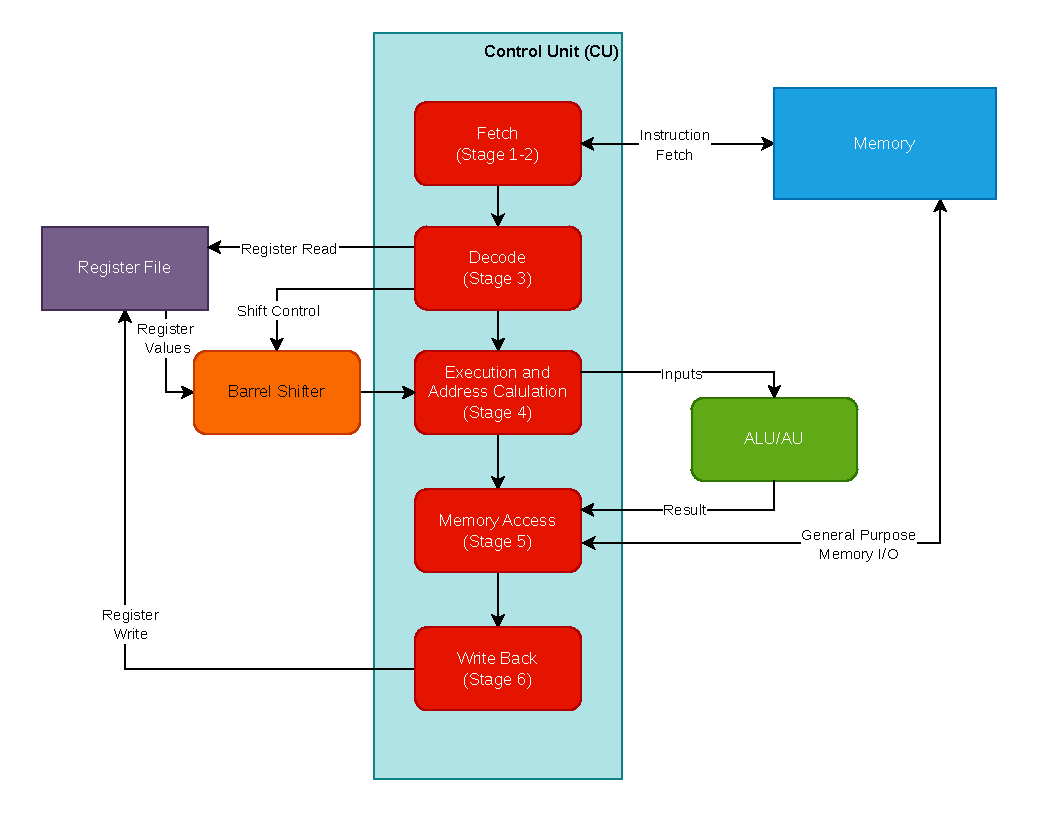
\includegraphics[width=\textwidth]{diagrams/cpu-block-diagram.pdf}
	\caption{SIRC-1 CPU Execution Phase Architecture}
	\label{fig:cpu-block-diagram}
\end{figure}

%TODO: Update the diagram so that the memory component is obviously separate to the other components that live together in the chip

\subsection{Control Unit (CU)}

The Control Unit sits at the heart of the SIRC-1 CPU, coordinating all other functional units throughout the
instruction execution phases. It decodes instructions and generates control signals that orchestrate data movement and
operations across the CPU.

Key responsibilities include:
\begin{itemize}
	\item Instruction fetch and decode
	\item Execution phase coordination
	\item Control signal generation for all functional units
	\item Condition code evaluation for conditional execution
\end{itemize}

\subsection{Arithmetic Logic Unit (ALU)}

The ALU performs all arithmetic and logical operations on register values. It supports the following operations:

\begin{itemize}
	\item \textbf{Arithmetic:} Addition, Subtraction (with and without carry)
	\item \textbf{Logical:} AND, OR, XOR
	\item \textbf{Comparison:} Test and compare operations
	\item \textbf{Status Flag Generation:} Carry, Overflow, Negative, Zero
\end{itemize}

The ALU operates exclusively on data from the Register File (after optional shifting) and outputs results either back
to the Register File or to memory via the data bus.

\subsection{Addressing Unit (AU)}

The Addressing Unit calculates memory addresses and manages address-related operations. It is responsible for:

\begin{itemize}
	\item Computing effective addresses from base + displacement
	\item Handling pre-decrement and post-increment addressing modes
	\item Updating address register pairs (l, a, s, p) for LDEA, jump, and branch instructions
	\item Presenting calculated addresses to the address bus
\end{itemize}

The AU works in parallel with the ALU during the execution stage, allowing address calculation to occur simultaneously
with ALU operations.

\subsection{Register File}

The Register File contains all CPU registers organized into three categories:

\begin{itemize}
	\item \textbf{General Purpose Registers:} \reg{r1}--\reg{r7}
	\item \textbf{Address Register Pairs:} \reg{l} (link), \reg{a} (address), \reg{s} (stack), \reg{p} (program counter)
	\item \textbf{Status Register:} \reg{sr}
\end{itemize}

The Register File provides multi-port access, allowing the ALU, AU, and Control Unit to read and write registers as
needed during each execution phase. All registers are 16 bits wide, though address register pairs can be combined to
form 24-bit addresses.

\subsection{Barrel Shifters}

A barrel shifter sits between the Register File and the CU, enabling efficient bit manipulation operations.

The barrel shifters support logical shift left (\mnemonic{LSL}), logical shift right (\mnemonic{LSR}), arithmetic shift
left (\mnemonic{ASL}), arithmetic shift right (\mnemonic{ASR}), rotate left (\mnemonic{RTL}), and rotate right
(\mnemonic{RTR}). Shift amounts can be specified as immediate values or dynamically from register contents.

The shift is applied to the first source operand when fetching the source registers for an instruction. Shifts cannot
be applied to the result or any other source operand.

\section{Design Characteristics}

\subsection{Combinatorial Logic Implementation}

The SIRC-1 uses pure combinatorial logic with no microcode engine. Each execution phase is implemented as combinatorial
circuits that process data in a single clock cycle. This approach:

\begin{itemize}
	\item Simplifies the hardware design
	\item Provides a deterministic, fixed execution sequence
	\item Eliminates the complexity of microcode sequencing
	\item Makes the CPU behavior fully predictable and easy to reason about
\end{itemize}

\subsection{Fixed Execution Sequence}

Ordinary instructions execute in exactly 6 phases, regardless of instruction type or operands, and complete in 6 clock
cycles when no bus wait states are required. Delayed bus acknowledgement can hold a phase and add wait cycles.
Coprocessor calls are the exception: the processing-unit instruction takes six cycles and the coprocessor dispatch that
follows takes a further six; DMA commands additionally hold instruction fetch until the transfer completes. This design
choice simplifies software timing and eliminates the need for branch prediction or complex multi-stage control logic
found in variable-time architectures.

\subsection{Parallel Functional Units}

The ALU and AU operate in parallel during phase 3 (Execute and Address Calculation), allowing address calculation to
proceed simultaneously with arithmetic operations. This parallelism enables efficient execution of memory reference
instructions without additional clock cycles.

\section{External Interface}

The SIRC-1 CPU exposes its bus, interrupt, and reset signals as physical pins; the chip package, the pin-by-pin descriptions, and the bus timing diagrams are given in Appendix~\ref{appendix:external-interface}. One architectural fact the rest of this chapter relies on: on \texttt{RSTI} assertion the CPU aborts the current instruction or bus wait and restarts at phase 0, as described in the six-stage execution phases above.
